\chapter{Lokalisation autonomer mobiler Robotersysteme}
\section{Abgrenzung: Lokalisation - Mapping - SLAM - Navigation}
\begin{itemize}
	\item \textbf{Lokalisation} Ermitteln der aktuellen Position des Roboters.
	\item \textbf{Kartenerstellung, Mapping oder Umgebungsmodellierung} hilft bei Entscheidung
	\subitem Kartenerstellung bedeuted die Auswertung der vom Roboter mittels Sensoren erfassten Daten der Umgebung mit dem Ziel, ein Umgebungsmodell zu erzeugne oder zu vervollständigen.
	\item \textbf{Großes Problem} Mapping
	\item \textbf{Pfadplanung oder Navigation} beantwortet die Frage \textbf{Wie gelange ich dorthin?} Bewegungsplanung oder Pfadplanung bedeutet die Berechnung der Fahrroute und der daraus abgeleiteten Bahn vom aktuellen Punkt zum Zielpunkt
	\item Man unterscheidet zwischen Navigation in unbekannter und in bekannter Umgebung.
	\item Selbstlokalisation und Kartenerstellung bedingen sich gegenseitig.
\end{itemize}
\section{Varianten der Selbstlokalisierung}
\paragraph{Lokale Selbstlokalisierung (position tracking)}
\begin{itemize}
	\item Die Startposition des Roboters ist ungefähr bekannt.
	\item Es handelt sich um \textbf{relative} Selbstlokalisierung
	\item Sobald sich der Roboter bewegt, muss aufgrund neuer Sensordaten die Position neu berechnet werden.
	\item Bezugspunkt ist der Startpunkt.
	\item \textbf{Methoden} Odometrie und Trägheitsnavigation
\end{itemize}
\paragraph{Globale Selbstlokalisierung}
\begin{itemize}
	\item Die Startposition ist unbekannt.
	\item Es handelt sich um \textbf{absolute Positionierung}
	\item An welcher Position der Roboter befindet, entscheidet er durch Auswerten seiner Sensordaten und durch erkennen von \textbf{signifikanten} Umgebungsmerkmalen
	\item \textbf{Mögliche Methode}: Triangulation
\end{itemize}
\paragraph{Kidnapped Robot Problem}
\begin{itemize}
	\item Die Position des Roboters ist anfangs bekannt
	\item Der Roboter wird willkürlich mit temporär deaktivierten Sensoren an eine beliebige andere Position versetzt, ohne darüber informiert zu werden.
	\item Auch dann muss das Verfahren robust die Position wiederfinden, zunächst muss der Roboter dies erkennen und sich dann relokalisieren
	\item Es muss eine erneute globale Lokalisierung durchgeführt werden
\end{itemize}
\section{Relative Lokalisierung versus Absolute Lokalisierung}
\paragraph{Relative Lokalisierung}
\begin{itemize}
	\item auch: \textbf{lokale}, \textbf{inkrementelle Lokalisierung} oder \enquote{tracking}
	\item Relativ zu einer Startpose wird sukzessiv die Änderung der Pose an diskreten, aufeinanderfolgenden Zeitpunkten ermittelt und integriert
\end{itemize}
\paragraph{Absolute Lokalisierung}
\begin{itemize}
	\item auch als \textbf{globale Lokalisierung} bezeichnet
	\item Die Pose wird in Bezug auf ein externes Bezugssystem ermittelt, z.B. einer Karte oder einem globalen Koordinatensystem
\end{itemize}
\paragraph{Ziel} Bestimme oder schätze die Position und Orientierung des Roboters in seiner Umgebung basieren auf
\begin{itemize}
	\item der Eigenbewegung
	\item durch Messungen der relativen Position zu unterscheidbaren Objekten in der Umgebung in Roboterkoordinaten (Ultraschall, Laser, Kamera)
\end{itemize}
%BSP Chapter 3 Seite 4 / 28 
\section{Transformation von Koordinatensystemen lokale <--> globale}
\paragraph{Kinematik} Die Kinematik ist die Lehre der Beschreibung von Bewegungen von Punkten im Raum. Dabei werden die Größen Weg, Geschwindigkeit und Beschleunigung betrachtet. Die Kinematik ist ein Teilgebiet der Mechanik.
\paragraph{Kinematische Robotermodell}
\begin{itemize}
	\item kreisförmiger Roboter
	\item Zweiradantrieb
	\item Bewegung in der Ebene
\end{itemize}
\paragraph{Lokales Koordinatensystem}
\begin{itemize}
	\item mit dem Roboter verbunden
	\item Ursprung in der Mitte der Antriebsachse
	\item x-Achse zeigt in Richtung des Roboterfrontteils
\end{itemize}
\paragraph{Festlegung der Roboterposition im globalen Koordinatensystem}
\begin{itemize}
	\item durch die Koordinaten $M(x_{M}, y_{M})$ im globalen Koordinatensystem
	\item durch den Winkel $\theta$ zwischen der lokalen x-Achse und der globalen x-Achse
	\item Pose p gegeben durch: p = $(x_M, y_M, \theta)^{T}$
\end{itemize}
\paragraph{Transformation von lokalen in globale Koordinaten}
\begin{itemize}
	\item Koordinaten von P im lokalen Koordinatensystem: $p_l=(x_l, y_l)^T$
	\item Koordinaten von P im globalen Koordinatensystem: $p_g = (x_g, y_g)^T$
	\item Transformation von $p_l$ nach $p_g(m=(x_M, y_M)^T: p_g=R(\theta)p_l)$
\end{itemize}
\paragraph{Transformation von globalen in lokale Koordinaten}
\begin{itemize}
	\item Transformation von globalen in lokale Koordinaten $p_l = R(\theta)^-1(p_g - m) = R(-\theta)(pg - m)$
\end{itemize}
\section{Karten für statistische und dynamische Umgebungen}
\begin{itemize}
	\item Generell gilt: \textbf{Karten} sollen eine explizite Repräsentation des Raumes sein.
	\item Die Karten sind auf die Sensorik des Roboters zugeschnitten
	\item Die Karten sind nicht vorrangig für den menschlichen Betrachter bestimmt, sondern der Roboter soll sie effizient nutzen können.
\end{itemize}
\paragraph{Statische Umgebungen}
\begin{itemize}
	\item basierend auf der Annahme, dass sich zwar der Zustand des Roboters innerhalb der Umgebung, nicht jedoch die Umgebung selbst ändert.
	\item Karte spiegelt die wirkliche Umgebung wider.
\end{itemize}
\paragraph{Dynamische Umgebungen}
\begin{itemize}
	\item Objekte können ihre Lage oder ihren Zustand ändern
	\item In der Karte registrierte Objekte können verschwinden, nicht registrierte Objekte auftauchen
	\item \enquote{Lernende} Karten sind ein fundamentales Problem in der mobilen Robotik
\end{itemize}
\subsection{Mapping Methoden}
\paragraph{Weltzentriert}
\begin{itemize}
	\item Die Pose aller Objekte einschließlich des Roboters werden in der Umgebung in Bezug auf ein festes Koordinatensystem repräsentiert.
	\item \textbf{Indoor}: Ursprung kann eine Zimmerecke sein
	\item \textbf{Outdoor}: Benötigung eines globalen Koordinatensystems, wie z.B. die Längen- oder Breitengrade, i.d.R. nutzen von \textbf{WGRS}(World Geographic Reference System)
\end{itemize}
\paragraph{Roboterzentriert} gebraucht um bspw. Kollisionen zu vermeiden
\begin{itemize}
	\item Durch Koordinaten-Transformation kann zwischen den verschiedenen Referenz-Frames konvertiert werden
\end{itemize}
\subsection{Arten von Modellen}
\begin{itemize}
	\item Die wichtigste Form von Umgebungsmodellen für mobile Roboter sind Umgebungskarten.
	\item Die folgende Ausführungen beziehen sich auf geeignet Karten für \textbf{mobile, autonome Landfahrzeuge}
\end{itemize}
\begin{figure}[H]
	\begin{center}
		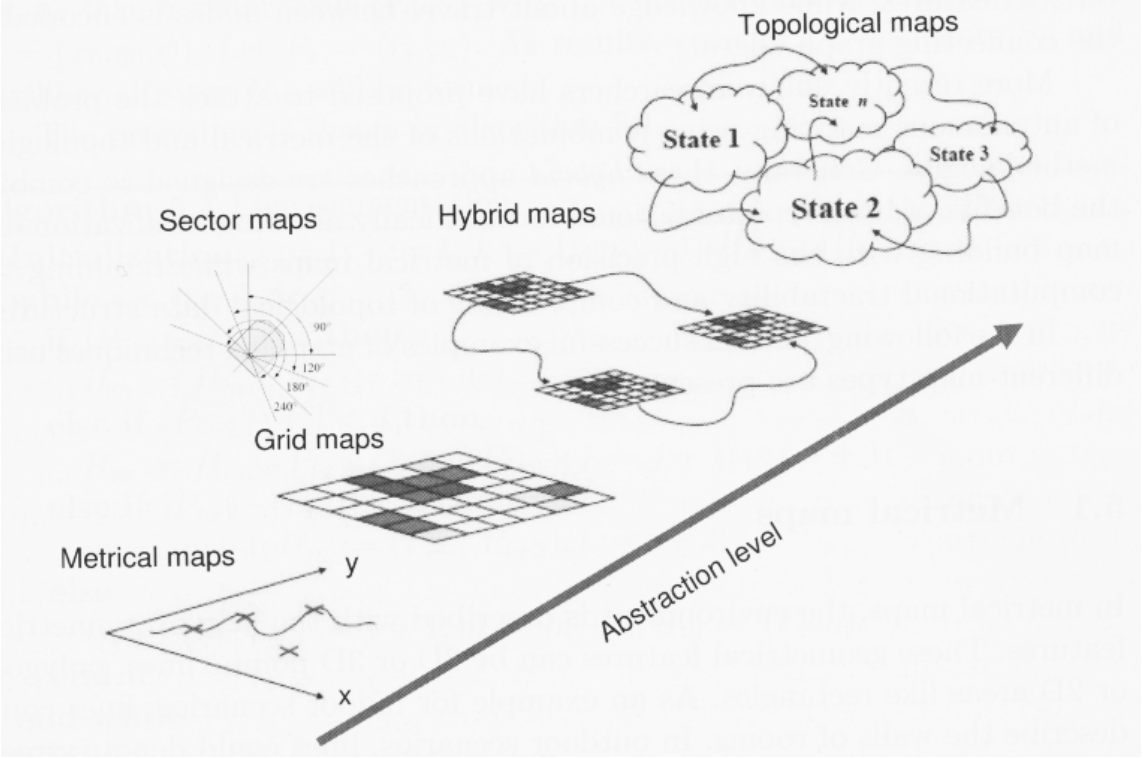
\includegraphics[scale=0.42]{Resources/PNG/MapTypes.PNG}
		\caption{}
		\label{fig:PNG/MapTypes.PNG}
	\end{center}
\end{figure}
\paragraph{Arten von Umgebungsmodellen}
\begin{itemize}
	\item \textbf{kontinuierliche metrische Karten}, zweidimensional oder dreidimensional:
	\subitem jedes Objekt wird assoziiert mit Koordinaten
	\item \textbf{diskrete metrische Karten, Grid Maps}, zweidimensional oder dreidimensional:
	\subitem der Raum wird gleichmäßig oder ungleichmäßig aufgeteilt; Objekte werden mit Positionen innerhalb des Gitters assoziiert
	\item \textbf{Hybrid Maps}
	\item \textbf{Topologische Modelle} nur zweidimensional
	\subitem im Vordergrund steht die Beziehung der Objekte zueinander
\end{itemize}
\subsection{Kontinuierliche Metrische Karten}
\begin{itemize}
	\item Metrische Lokalisierung, beruht auf Ultrashall oder Laserscannern
	\item Exakte Beschreibung der Umgebung mit 2D oder 3D Modellen möglich
	\item Die Positionen von Objekten der Umgebung werden durch ein Koordinatensystem repräsentiert.
	\item \textbf{Vorteil}: detailliertes Bild der Umgebung
	\item \textbf{Nachteil}: große, unstrukturierte Datenmengen erschweren die Pfadplanung
\end{itemize}
\subsection{Grid Maps - Rasterkarten}
\begin{itemize}
	\item Die Umwelt des Roboters wird in ein gleichmäßiges Raser oder Grid zerlegt.
	\item Jede Zelle enthält den Belegtheitsgrad der Zelle $\Rightarrow$ zeigt an ob zelle mit einem Hindernis belegt ist oder nicht
	\item Verschiedene Modelle verwenden unterschiedliche Werte
	\subitem zwei Werten
	\subitem freie Zellen, belegte Zellen und Zellen mit Mischbelegung
	\subitem Prozentsatz der Belegungswahrscheinlichkeit
	\item Notwendige Informatinoen sind z.B.:
	\subitem x, y als Koordinaten (Zeile, Spalte) einer Zelle
	\subitem Sensordaten des Roboters
	\subitem ein boolscher Wert für den Zustand der Zelle
	\item Die Werte in den Zellen sind unabhängig voneinander
	\item Eine Steigerung der Messgenauigkeit der Sensoren führt dazu, dass die Rasterelemente immer kleiner werden
	\item Für eine kompakte Notation können Grid Maps im 2-dimensionalen Raum mit Quadtrees im 3-dimensionalen mit Octtrees gespeichert werden
\end{itemize}
\paragraph{Gleichmäßige Gitterstruktur vs. Adaptiver Gitterstruktur}
\begin{figure}[H]
	\begin{center}
		\includegraphics[scale=0.5]{Resources/PNG/Quadtrees.PNG}
		\caption{}
		\label{fig:PNG/Quadtrees.PNG}
	\end{center}
\end{figure}
\begin{itemize}
	\item links oben zeigt die Objekte in einer gleichmäßigen Gitterstruktur
	\item rechts oben zeigt die zugehörige Repräsentation über Belegtheiten der Zellen
	\item speicherintensiv bei gleichmäßiger Unterteilung des Raums $\Rightarrow$ adaptive Unterteilung des Raums und Speicherung in Quadtrees oder bei 3. Dimension Octtrees
\end{itemize}
\subsection{Adaptive Unterteilung}
\begin{itemize}
	\item Ausgangszustand: Rechteck mit Hindernissen
	\item Fläche wird unterteilt in 4 Rechtecke gleicher Größe
	\item Jedes Rechteck wird rekursiv wieder in 4 Rechtecke unterteilt $\Rightarrow$ Quadtree
	\item Attributierung der Knoten:
	\subitem \textbf{Frei}: Rechteck enthält keinen Teil eines Hindernisses
	\subitem \textbf{Belegt}: Rechteck ist vollständig von Hindernis belegt
	\subitem \textbf{Gemischt}: Rechteck enthält Punkte, die zu einem Hindernis gehören, sowie solche die es nicht tun
	\item Nur gemischte Knoten werden weiter unterteilt
\end{itemize}
\paragraph{Vorteile} schnell und leicht feststellbar, ob Punkt in einem Hindernis liegt
\paragraph{Nachteile} 
\begin{itemize}
	\item Konturen der Objekte und der Freiraum zwischen ihnen wird unpräzise repräsentiert
	\item Um die Datenfülle zu reduzieren, wird das Raster zu grob gewählt und dadurch ein möglicher Weg durch Mischpixel versperrt
\end{itemize}
\paragraph{Weiterer Verwendungszweck}
Neben der reinen Lokalisierung können die Karten auch dazu verwendet werden eine Fahrspur (Trakektorie) zu berechnen.
\begin{figure}[H]
	\begin{center}
		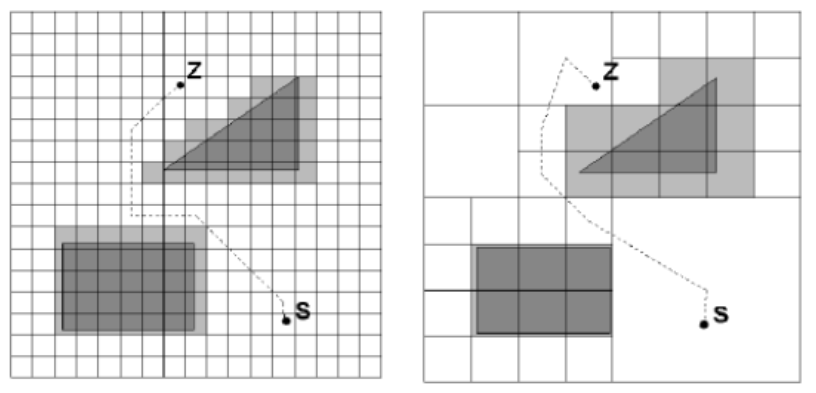
\includegraphics[scale=0.5]{Resources/PNG/Trajektorie}
		\caption{}
		\label{fig:PNG/Trajektorie}
	\end{center}
\end{figure}
\subsection{Weitere Beispiele für Umgebungskarten}
\begin{itemize}
	\item Laserscan Karten
	\item Bildbasierte Karten
\end{itemize}
\subsection{Topologische Karten}
Bedingt geeignet zur Lokalisation, Haupteinsatzgebiet ist die Pfadplanung.
\begin{figure}[H]
	\begin{center}
		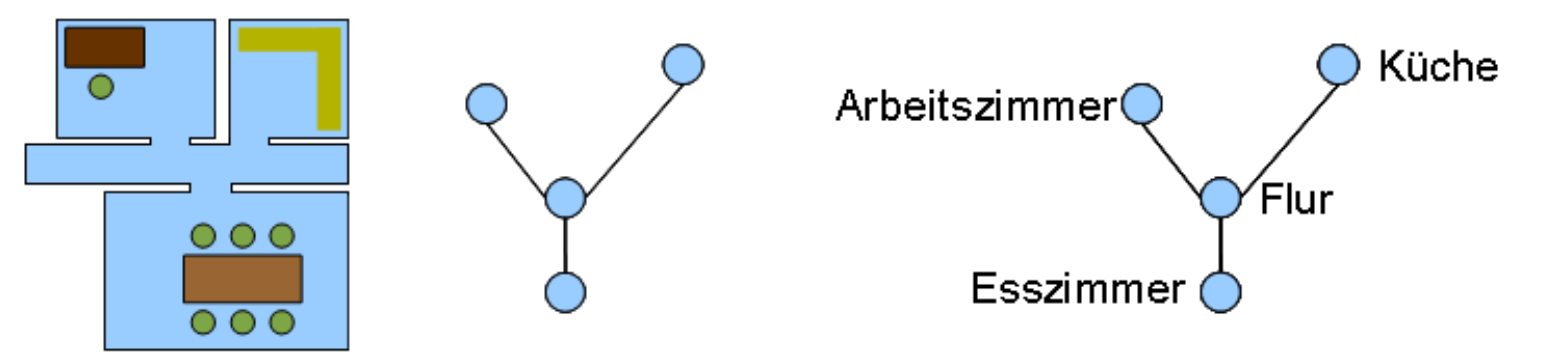
\includegraphics[scale=0.42]{Resources/PNG/TopologischeKarte.PNG}
		\caption{}
		\label{fig:PNG/TopologischeKarte.PNG}
	\end{center}
\end{figure}
\begin{itemize}
	\item Modelle bilden einen \textbf{Graphen}
	\item \textbf{Knoten} entsprechen Orten oder Bereichen der Umgebung
	\item Beziehungen zwischen den Orten werden durch \textbf{Kanten} modelliert.
	\item Zwei Knoten sind durch eine Kante verbunden, wenn sie unmittelbar voneinander erreichbar sind.
	\item \textbf{Gewichte}: Maß für die Länge der Wege
	\item Ist die Länge der jeweiligen Wegstücke bekannt, lässt sich der kürzeste Weg finden.
\end{itemize}
\paragraph{Vorteile}
\begin{itemize}
	\item Kompaktheit
	\item Gute Skalierbarkeit für welträumige Umgebungen.
	\item Es gibt viele schnelle Algorithemn auf Graphen, die gut zur Pfadplanung eingesetzt werden können
\end{itemize}
\paragraph{Nachteil} Relevante Umgebungsmerkmale werden verdeckt. Landmarken werden schwerer erkannt.
\subsection{Hybrid Maps}
\begin{itemize}
	\item Kombinieren metrische und topologische Ansätze
	\item Ermöglichen Lokalisation und Kantenerstellung mit hoher Präzision
	\item Erhalten die Kompaktheit der topologischen Ansätze
\end{itemize}
\paragraph{Abstraktions-basierter Ansatz}
\begin{itemize}
	\item Basis: konstruieren einer metrischen Karte der Umgebung
	\item $\Rightarrow$ aufbau einer kompakten topologischen Repräsentation
	\item \textbf{Vorteil} Effizient Planung eines Pfads zu einem gegebenen Ziel aufgrund der Abstraktion.
	\item Die zugrunde liegende metrische Karte wird für Relokalisation und Hindernisvermeidung benötigt.
\end{itemize}





































